\documentclass[]{standalone}

\usepackage{amsmath}
\usepackage{amsfonts}
\usepackage{amssymb}
\usepackage{graphicx}
\usepackage{tikz}
\usepackage{import}
\usepackage[subpreambles=true]{standalone}

\usepackage{tikz}
\usepackage{tikz-3dplot}

\usetikzlibrary{positioning}
\usetikzlibrary{calc}
\begin{document}

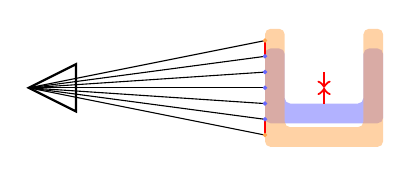
\begin{tikzpicture}[scale=1]
    \coordinate (camera) at (0, 0);
    \coordinate (virtual) at (3, 0.75);
    \coordinate (object) at (3, 0.5);
    \coordinate (grid) at (2.5, 0.5);

    \begin{scope} [transparency group, opacity=0.5, rotate=0,shift={(object)}]
        \path[rounded corners=2pt, fill=blue!60] (0,0) -- ++(0.25,00) -- ++(0,-0.7) -- ++(1.0, 0) -- ++(0,0.7) -- ++(0.25,0) -- ++(0,-0.95) -- ++(-1.5,0) -- cycle;
    \end{scope}

    \begin{scope} [transparency group, opacity=0.5, rotate=0,shift={(virtual)}]
        \path[rounded corners=2pt, fill=orange!70] (0,0) -- ++(0.25,00) -- ++(0,-1.25) -- ++(1.0, 0) -- ++(0,1.25) -- ++(0.25,0) -- ++(0,-1.5) -- ++(-1.5,0) -- cycle;
    \end{scope}

    \draw[thick, red, ->] (virtual) ++ (0.75,-0.55) -- ++(0,-0.2);
    \draw[thick, red, ->] (virtual) ++ (0.75,-0.95) -- ++(0,+0.2);

% \draw[step=0.25cm,black,thin,xshift=0.0cm,yshift=0.0cm,gray] ($(grid)-(0.001,-0.001)$) grid ++(4.001,-4.001);
% \def\d1{0.5}

    \begin{scope} [rotate=0,shift={(camera)}]
        % \path[draw, thin, red] (3,0) -- (3.25,0);
        % \path[draw, thin, red] (3,0.2) -- (3.25,0.2166);
        % \path[draw, thin, red] (3,0.4) -- (3.25,0.4333);
        % \path[draw, thin, red] (3,0.6) -- (3.25,0.65);
        % \path[draw, thin, red] (3,-0.2) -- (3.25,-0.2166);
        % \path[draw, thin, red] (3,-0.4) -- (3.25,-0.4333);
        % \path[draw, thin, red] (3,-0.6) -- (3.25,-0.65);
        \path[draw, thin] (0,0) -- (3,0);
        \path[draw, thin] (0,0) -- (3,0.2);
        \path[draw, thin] (0,0) -- (3,0.4);
        \path[draw, thin] (0,0) -- (3,0.6);
        \path[draw, thin] (0,0) -- (3,-0.2);
        \path[draw, thin] (0,0) -- (3,-0.4);
        \path[draw, thin] (0,0) -- (3,-0.6);
        \path[draw, thick] (0,0) -- (0.6,0.3) -- (0.6, -0.3) -- cycle;

        \draw[fill, thin, red] (3,0.6) -- (3,0.4);
        \draw[fill, thin, red] (3,-0.6) -- (3,-0.4);

        \draw[fill, blue!60] (3,0) circle (0.02);
        \draw[fill, blue!60] (3,0.2) circle (0.02);
        \draw[fill, blue!60] (3,0.4) circle (0.02);
        % \draw[fill, blue!60] (3,0.6) circle (0.02);
        \draw[fill, blue!60] (3,-0.2) circle (0.02);
        \draw[fill, blue!60] (3,-0.4) circle (0.02);
        % \draw[fill, blue!60] (3,-0.6) circle (0.02);
        % \draw[fill, orange!70] (3,0) circle (0.02);
        % \draw[fill, orange!70] (3,0.2) circle (0.02);
        % \draw[fill, orange!70] (3,0.4) circle (0.02);
        \draw[fill, orange!70] (3,0.6) circle (0.02);
        % \draw[fill, orange!70] (3,-0.2) circle (0.02);
        % \draw[fill, orange!70] (3,-0.4) circle (0.02);
        \draw[fill, orange!70] (3,-0.6) circle (0.02);
    \end{scope}
\end{tikzpicture}
\end{document}
